
%
%  $Description: Author guidelines and sample document in LaTeX 2.09$ 
%
%  $Author: ienne $
%  $Date: 1995/09/15 15:20:59 $
%  $Revision: 1.4 $
%

\documentclass[10pt,twocolumn]{article} 
\usepackage{latex8}
\usepackage{listings}
\usepackage{graphicx}

%\documentstyle[times,art10,twocolumn,latex8]{article}

%------------------------------------------------------------------------- 
% take the % away on next line to produce the final camera-ready version 
\pagestyle{empty}

\newcommand{\url}[1]{\textsf{#1}}
\newcommand{\code}[1]{\lstinline{#1}}
\newcommand{\csharp}{C{\normalfont \#}}
\newcommand{\comment}[1]{}
\newcommand\codefamily\sffamily
\lstset{language={[Sharp]C},mathescape=true,flexiblecolumns=true,morekeywords={alloc,delay,delete,expose,let,unsatisfiable,receive,rep,contract,message,state,one},basicstyle=\codefamily\small,literate={->}{{$\rightarrow$}}{2}{<<}{{$\langle$}}{2}{>>}{{$\rangle$}}{2}{!}{{\textbf{!}}}{2},frame=lines,moredelim=[is][\itshape]{@}{@},captionpos=b,numberstyle=\tiny,stepnumber=1,numbersep=2pt}

%------------------------------------------------------------------------- 
\begin{document}

\title{Code Contracts for .NET: Better Contracts Make Better Neighbors} 

\author{Mike Barnett, Manuel F\"ahndrich, and Francesco Logozzo\\
Microsoft Research, One Microsoft Way, Redmond, WA, 98052-6399, USA\\
{\tt \{mbarnett, maf, logozzo\}@microsoft.com}\\
}

\maketitle
\thispagestyle{empty}

\begin{abstract}
Code Contracts for .NET provides a complete infrastructure and toolset for describing
component API specifications.
Using a library-based approach, all .NET languages can express method preconditions
and postconditions, even for interfaces and abstract types.
Exisiting tools provide runtime checking, static checking, automatic documentation generation,
and editor enhancements.
There is open-source support for manipulating contracts in an easy-to-use object model.
\end{abstract}
\vspace*{-5mm}

%------------------------------------------------------------------------- 
\Section{Introduction}
Components are effective only when it is possible to describe their interfaces
in a discoverable manner --- by both humans and machines.
For humans, it is crucial to have support for programming against a component:
knowing what methods to call and how to call them.
For machines, it is crucial to be able to verify --- either at runtime or
statically or a combination of the two --- whether a component meets its
specification.
Almost all existing languages and developer environments (IDEs) provide
such support, but only at the level of method names and the types of method
parameters.
These API (Application Programming Interface) specifications are the boundaries
of each component.
Such ``fences'' make for good neighbors:
programmers use the editor support
when writing their programs and compilers and linkers use the type signatures
to prevent errors.

We propose to increase the expressivity of specifications to include
more than just type information.
Over the past several years we have developed Code Contracts for .NET, a
library-based approach for describing method preconditions and postconditions
and also object invariants.
We have created tools that make use of the contracts, for humans and for
machines:
\begin{itemize}
\item Runtime checking
\item Static verification
\item Automatic documentation generation
\item Editor enhancements
\end{itemize}
The tools have been freely available since February 2009 and have been downloaded more than 20,000 times.
Part of the infrastructure have already shipped as an integral part of .NET 4.0 and other parts
are available for open-source development.

In this paper, we provide an overview of the overall project, the contract ``language'', and
the existing tools.
We hope to encourage a community using our shared infrastructure to develop further
tools in order to provide better support for components in .NET.

%------------------------------------------------------------------------- 
\Section{Contract Expressivity}
Contracts are written as method calls to a set of static methods defined
in the class {\tt Contract}, which is defined in the namespace {\tt System.Diagnostics.Contracts}.
The namespace and class were introduced in the .NET Base Class Library (BCL)
in version 4.0.
Support for previous versions of .NET are provided through a separate library
comprising the contract class methods.

An example using \csharp{} is shown in Figure~\ref{fig:csharp}.
\begin{figure}[thb]
\begin{small}
\begin{lstlisting}
int Increment(int value, string label) {
  Contract.Requires( value > 0 );
  Contract.Requires( label != null );
  Contract.Ensures( Count == 
                    Contract.OldValue(Count) + value );
  Contract.Ensures( Contract.Result<int>()
                    == Contract.OldValue(Count) );
  ...
\end{lstlisting}
\caption{An Increment specification in \csharp}
\label{fig:csharp}
\end{small}
\end{figure}
Preconditions and postconditions are expressed as calls to the static
methods \lstinline{Contract.Requires} and
\lstinline{Contract.Ensures}. Special dummy methods are used to refer
to the method's return value as well as referring to the \emph{old}
value of an expression, meaning the value of the expression on method
entry.
Note that the arguments to the contract methods are just written in
ordinary \csharp{} syntax.
If the program had been written in VB, then the contract methods would
stay the same, but their arguments would be the equivalent VB code.

Such a language-agnostic approach has many advantages: 
\begin{itemize}
\item Developers need not learn a new language for
specifications. Predicates are boolean conditions expressed in the
source language.
\item No new front-ends or compilers are required. Standard compilers directly translate contracts into
  .NET intermediate language (MSIL). As a benefit, compilers
  check the syntax and typing of contract conditions, thus avoiding errors in specifications,
  such as unresolved names, that would arise if the specifications
  were written in comments or attributes.
\item Standard development environments help writing
  specifications in the same way they help writing other code, via highlighting, intellisense,
  completion, etc.
\item The semantics of contracts is defined by that the semantics of the generated MSIL. 
  The compiled code acts as a persisted format of specifications consumable by a variety of tools.
\end{itemize}
The language independence extends from the specification language to
the tools themselves as they consume the output of each language's compiler.

%------------------------------------------------------------------------- 
\Section{Runtime Contract Checking}
In a post-build step, the compiled binaries containing the calls to the contract
methods are transformed by having each specification injected at the 
appropriate program points.
For instance, method postconditions are moved to the exit points of each method
and calls to Contract.Result are replaced with the return value of the method.
At the beginning of each method, arguments to Contract.OldValue are evaluated and
stored into locals which then replace those method calls within the postcondition-checking
code.

In addition, contracts from supertypes and interfaces are inherited by subtypes
and interface implementations. This provides the basis for enforcing behavioral
subtyping \cite{Liskov-Wing94}, which is required for modular checking.

%------------------------------------------------------------------------- 
\Section{Static Checking}
Our static checker is based on abstract interpretation rather than
SMT solvers traditionally used for program verification, in order to
automate the generation of loop
invariants and strongest postconditions.

Although we use modular verification which, in principle, requires
specifications at all method boundaries, we use techniques to infer
pre- and postconditions whenever possible.

The existing abstract domains provide an analysis that checks for
null dereferences, array indexing, arithmetic overflow, in addition
to user-defined general properties.

%------------------------------------------------------------------------- 
%------------------------------------------------------------------------- 
%------------------------------------------------------------------------- 
%------------------------------------------------------------------------- 

\begin{figure*}[tb]
\begin{center}
  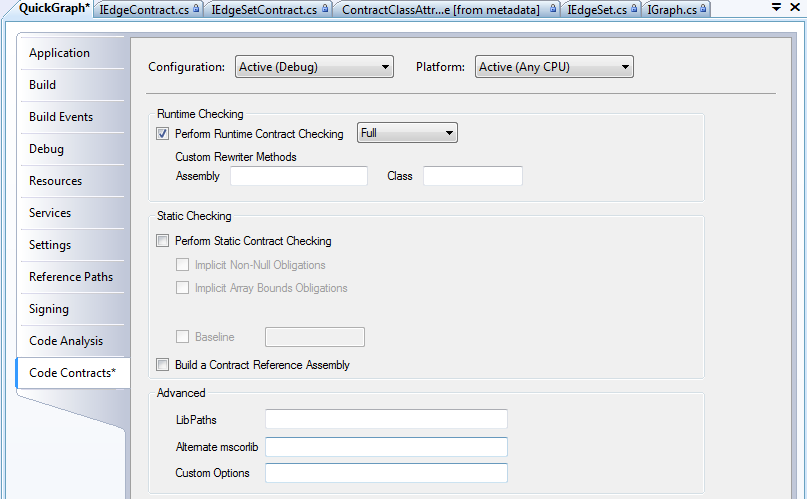
\includegraphics[width=2\columnwidth]{ContractUI.png}
\end{center}
\caption{The Code Contact User Interface}
\label{fig:contractui}
\end{figure*}

\begin{figure}[thb]
\begin{small}
\begin{lstlisting}
Function Increment(ByVal value As Integer) As Integer
  Contract.Requires( value > 0 )
  Contract.Requires( label IsNot Nothing )
  Contract.Ensures( Count
                    = Contract.OldValue(Count) + value )
  Contract.Ensures( Contract.Result(Of Integer)()
                    = Contract.OldValue(Count) )
  ...
\end{lstlisting}
\end{small}
\caption{An Increment specification in Visual Basic}
\label{fig:vb}
\end{figure}

\section{Screenshots}
Figure~\ref{fig:contractui} shows the contract user interface in
Visual Studio. The UI allows the programmer to enable runtime checking
and/or static checking. The integration in the IDE manages all the
extra build steps transparently.

As an example of the language-agnostic approach, the same
specification as in Figure~\ref{fig:csharp} can be written in Visual
Basic as shown in Figure~\ref{fig:vb}.

\begin{figure}[htb]
\begin{center}
  \includegraphics[width=\columnwidth]{FoxtrotOutput.png}
\end{center}
\caption{Example of Runtime Contract Failure}
\label{fig:foxtrot}
\end{figure}

\begin{figure*}[tb]
\begin{center}
  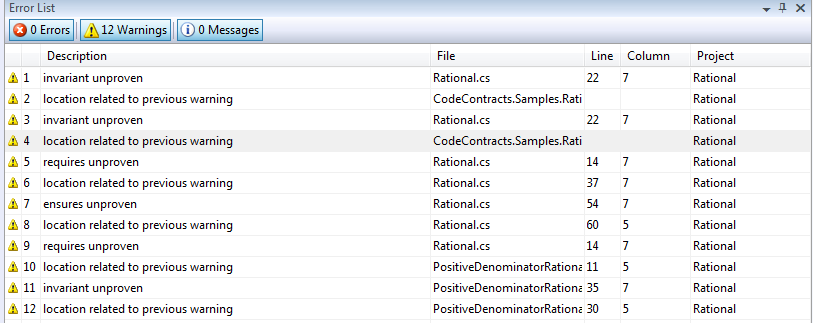
\includegraphics[width=2\columnwidth]{staticCheckerOutput.png}
\end{center}
\caption{Example of Static Checker Output}
\label{fig:clousot}
\end{figure*}

Figure~\ref{fig:foxtrot} shows the default contract failure behavior
when runtime checking of contracts is enabled. In this case, an
invariant was violated.

Figure~\ref{fig:clousot} shows the output produced by a run of the
static contract verifier.


\bibliographystyle{latex8}
\bibliography{bib}

\end{document}

